\chapter{Local continuation methods}\label{chap2} % chapter II  

\section{Introduction}\label{chap2-sec2.1}\pageoriginale
  
We will use a local continuation method to get global solutions of the
general problem:  
\begin{equation*}
G(u, \lambda) = 0 \tag{2.1}\label{chap2-sec2.1-eq2.1}
\end{equation*}

Suppose we are given a solution $(u^{o}, \lambda^{o})$ of
\eqref{chap2-sec2.1-eq2.1}. The 
idea of local continuation is to find a solution at
$(\lambda^{o}+\delta \lambda)$ for a small perturbation $\delta
\lambda$. Then perhaps, we can proceed step by step, to get a global
solution. The basic tool for this study is the implicit function
theorem.The continuation method may fail at some step because of the
existence of singularities on the curve (for example folds or
bifurcation points). Near these points there exist more than one
solution and the implicit function theorem is {\em not} valid.  

First we recall a basic theorem which is the main tool in proving the
implicit function theorem.  

\section{Contraction Mapping Theorem}\label{chap2-sec2.2} 

\textit{Let $B$ be a Banach space and $F : B \to B$
satisfy}:  
\begin{equation*}
  \begin{array}{r@{\;\;}>{$}p{6.5cm}<{$}}
\text{(a)} &  F (\bar{\Omega}) \subset \bar{\Omega} \textit{ for some
  closed subset } 
\bar{\Omega} \subset B.\\ 
\text{(b)} & \| F (u)-F(v) \| \le \theta \| u-v\| \textit{ \ for
  some \ }\theta \in (0,1) \textit{ \ and for all \ } u, v \in \bar{\Omega}. 
\end{array}\tag{2.2}\label{chap2-sec2.2-eq2.2} 
\end{equation*}

\textit{Then\pageoriginale the equation
$$
u = F(u)
$$
has one and only one solution  $u^{*} \in \bar{\Omega}$. 
This solution is the limit of any sequence $\{u_{U}\}$, $U = 0, 
1,2,\ldots$ generated by} 
\begin{equation*}
\begin{array}{r@{\;\;}l}
\text{(a)} & u_{o} \in \bar{\Omega}, \text{ \ arbitrary;}\\  
\text{(b)} & u_{U+1} = F(u_{U}), U = 0,1,2, \ldots \ldots
\end{array}
\tag{2.3} 
\label{chap2-sec2.2-eq2.3} 
\end{equation*}

\textit{The convergence is such that}:
\setcounter{equation}{2}
\begin{equation*}
\text{(c)~ }  \|u^{*} - u_{U}\| \le \frac{\theta^{U}}{1-\theta} \|
u_{o} - F(u_{0})\| \equiv \frac{\theta^{U}}{1-\theta} \| u_{0} -
u_{1}\|.  \tag{2.3}\label{chap2-sec2.2-addeq2.3} 
\end{equation*}

\begin{proof}
Well known
\end{proof}

We will state another lemma which shows how to find a set $\bar{\Omega}$, in
which the conditions of theorem \eqref{chap2-sec2.2} hold. 


\setcounter{section}{3}
\section{Contracting Ball Lemma}\label{chap2-sec2.4} 

\textit{Let $\rho > 0$, $\theta \in (0,1)$  be such that for
  some $u_{o} \in B$, $F$ satisfies:} 
\begin{equation*}
\begin{array}{r@{\;\;}l}
\text{(a)} & \|u_{o}-F(u_{o})\| \le (1-\theta) \rho.\\ 
\text{(b)} & \|F(u) - F(v)\| \le \theta \| u-v\| \textit{ \ for
  all \ }, u, v \in \bar{B}_{\rho}(u_{o}). 
\end{array}
\tag{2.4}\label{chap2-sec2.4-eq2.4} 
\end{equation*}
\textit{where}
$$
\bar{B}_{\rho}(u_{o}) = \{u \in B : \| u-u_{o}\| \le \rho\}. 
$$

\textit{Then the conditions \eqref{chap2-sec2.2-eq2.2}  of theorem
  \eqref{chap2-sec2.2} hold with $\bar{\Omega} = \bar{B}_{\rho}(u_{o})$.} 

\begin{proof}
For any $u \in \bar{B}_{\rho}(u_{o})$, 
$$
\|F(u) - u_{o}\| \le \|F(u) -F(u_{o})\| + \|F(u_{o}) - u_{o}\| \le
\theta \rho+ (1-\theta)\rho = \rho, 
$$
which proves (a) of \eqref{chap2-sec2.2-eq2.2}. Part (b) of
\eqref{chap2-sec2.2-eq2.2} is trivial 
\end{proof}

\section{Fundamental Theorem of Calculus}\label{chap2-sec2.5}
\pageoriginale%%% 2.5 

\textit{Let $F$ be a differentiable operator defined on a
  Banach space $B$. Then for all $u$, $v \in B$:}
\begin{equation*}
F(u) - F(v) = \int\limits^{1}_{0} \frac{d}{dt} F(tu+(1-t)v)dt
\tag{2.5}\label{chap2-sec2.5-eq2.5}   
 \end{equation*} 

We have on differentiating
$$
\frac{d}{dt} F(tu+(1-t)v) = F_{u}(tu+(1-t)v) (u-v), 
$$
and if we see
$$
\tilde{F}_{u}(u,v) \equiv \int\limits^{1}_{0} F_{u}(tu+(1-t)v)\,dt 
$$
then we obtain the mean value formula :
\begin{equation*}
F(u) - F(v) = \tilde{F}_{u} (u,v)
(u-v). \tag{2.6}\label{chap2-sec2.5-eq2.6}    
\end{equation*} 

This is valid provided $F$ is differentiable on the ``line" joining
$u$ and~$v$. 
 
Now we will state and prove:

\setcounter{section}{6}
\section{Implicit Function Theorem}\label{chap2-sec2.7}%%% 2.7 

\textit{Let $G : B_{1} \times  B_{2} \to B_{1}$ satisfy for
   some $\rho_{1} > 0$, $\rho_{2} > 0$, sufficiently small,
 ($B_{1}$ is a Banach space and $B_{2}$ is the parameter space, 
either\pageoriginale it is Euclidean space or more generally it can be a Banach
space) the following conditions:} 
\begin{equation*}
\centering
\begin{array}{r@{\;\;}>{$}p{9cm}<{$}@{}}
\text{(a)} & G (u^0, \lambda^0) = 0 \text{ \ for some \ }
u^0 \in B_1, \lambda^0 \in B_2.\\ 
\text{(b)} & G^0_u \equiv G_u (u^0, \lambda^0)
\text{ \ is nonsingular with a bounded}\newline
\text{inverse, i.e.~: \ } \|
(G^0_u)^{-1} \| \le~M_0,~\text{for some constant } M_0.\\ 
\text{(c)} & G (u, \lambda ) \text{ and } G_u (u,
\lambda ) \text{ \ are continuous on \ } B_{\rho_1}(u^0)~\times~B_{\rho_2}(\lambda^0).
\end{array}\tag{2.7}\label{chap2-sec2.7-eq2.7}    
\end{equation*}


\textit{Then for all $\lambda \in
B_{\rho_2}(\lambda^0)$, there exists  $u(\lambda) \in B_{\rho_1}(u^0)$ 
such that:} 
\begin{equation*}
\begin{array}{r@{\;\;}>{$}p{8.5cm}<{$}}
\text{(d)} & u(\lambda^0) = u^0.\\  
\text{(e)} & \text{Existence~:} G(u(\lambda), \lambda) =
0.\\ 
\text{(f)} & \text{Uniqueness~: For \ } \lambda~\in~B_{\rho_2}(\lambda^0) \text{ \ there is no solution of}\newline  
G(u, \lambda ) = 0 \text{ \ in \ } B_{\rho_1}(u^0) 
\text{ \ other than \ } u(\lambda).\\   
\text{(g)} & \text{Continuous dependence~: } u(\lambda)
  \text{ \ is continuous on \ }\newline B_{\rho_2}(\lambda^0)  \text{
    \ and has, upto a factor, the same modulus}\newline \text{of
    continuity with respect to \ } \lambda, \text{ \ as\ } G(u, \lambda). 
\end{array}\tag{2.7}\label{chap2-sec2.7-addeq2.7}    
\end{equation*}

\begin{proof}
Since $G^0_u$ is nonsingular, it follows that: 
$$
G^0_u u = G^0_u u - G(u, \lambda)  \text{ \ if and only if \ } 
G(u,\lambda) = 0. 
$$
\end{proof}

Hence $G(u,\lambda) = 0$ is equivalent to :
\begin{equation*}
u = (G^0_uu)^{-1} [G^0_u u - G(u, \lambda)] \equiv F(u, \lambda)
\tag{2.8}\label{chap2-sec2.7-eq2.8}     
\end{equation*}

Thus the problem of solving $G(u, \lambda) = 0$ reduces to finding the
fixed point of the operator $F(u, \lambda)$ for a given $\lambda$.
Note that $u^0$ is a fixed point for $\lambda = \lambda^0$. 

Next, we will check the conditions (a) and (b) of the contracting
ball\pageoriginale lemma \eqref{chap2-sec2.4} so that we can apply the
contraction mapping 
theorem \eqref{chap2-sec2.2}. Take any $\lambda \in
B_{p_2}(\lambda^0)$ and use 
$F(u^0, \lambda^0) = u^0$, to get: 
\begin{align*}
\| u^0 - F(u^0, \lambda) \| & =\|F(u^0, \lambda^0) - F(u^0, \lambda) \| \\
& \le M_0 \| G(u^0, \lambda) - G(u^0, \lambda^0) \| \\
& \le M_0 \omega_0 (\mid \lambda^0 - \lambda \mid ).
\end{align*}

Thus we have
\begin{equation*}
\| u^0 - F(u^0, \lambda) \| \le M_0 \omega_0
(p_2). \tag{2.9}\label{chap2-sec2.7-eq2.9}      
\end{equation*}

Here we have introduced the modulus of continuity $\omega_0$ defined
as: 
\begin{gather*}
\omega_0 (\rho) = \sup_{\left \{ 
\begin{matrix}
\| \lambda - \tilde{\lambda} \| \le \rho ,\\
\lambda,\tilde{\lambda} \in B_{\rho_2} (\lambda^0) ,\\
u, v \in B_{\rho_1} (u^0). 
\end{matrix}
\right \}} \| G(u,\lambda) - G(v, \tilde{\lambda}) \|. \tag{2.10} 
\label{chap2-sec2.7-eq2.10}    
\end{gather*}
$\omega_0$ is nonnegative and nondecreasing and also $\omega_0 (\rho)
\rightarrow 0 $ as $\rho \rightarrow 0$ by
(\ref{chap2-sec2.7-eq2.7}c). Next fo $u$, $v \in B_{\rho_1} (u^0)$, we have: 
\begin{align*}
F(u, \lambda) -F(v, \lambda) &= (G^0_u)^{-1} [G^0_u (u-v) - (G(u,
  \lambda) - G(v, \lambda))], \\ 
&  = (G^0_u)^{-1} [G^0_u - \tilde{G_u} (u, v, \lambda)] (u-v),
\tag{2.11a} \label{chap2-sec2.7-eq2.11a}    
\end{align*}    
where,
$$ 
\tilde{G_u} (u, v, \lambda) = \int\limits^1_0 G_u (tu + (1-t) v,
\lambda) dt.  
$$

Thus we have:
\begin{align*}
G^0_u - \tilde{G_u} (u, v, \lambda) & = \int \limits^1_0 [G_u - G_u
  (tu + (1-t) v, \lambda)] dt, \\ 
& = \int \limits^1_0 [G_u (u^0 , \lambda^0)  - [G_u (u^0, \lambda) +
    [G_u (u^0, \lambda) \\  
&   \qquad \qquad -  G_u (tu + (1-t) v, \lambda)] dt.\tag{2.11b}  
\label{chap2-sec2.7-eq2.11b}    
\end{align*}

But\pageoriginale 
\begin{equation*}
\| G_u (u^0, \lambda^0 - G_u (u^0, \lambda) \| \le \omega_2 (\rho_2),
\tag{2.11c}\label{chap2-sec2.7-eq2.11c}     
\end{equation*}
and 
\begin{equation*}
\| G_u (u^0, \lambda - G_u (tu + (1-t)v, \lambda) \| \le \omega_1
(\rho_1), \tag{2.11d}\label{chap2-sec2.7-eq2.11d}     
\end{equation*}
where we have introduced the moduli of continuity $\omega_1$ and
$\omega_2$ as : 
$$
\omega_1 (\rho_1) = \sup_{\left \{ 
\begin{matrix}
\| \lambda \in B_{\rho_2} (\lambda^0) \\
w, \in B_{\rho_1} (u^0),  
\end{matrix}
\right \}} \| G(u^0 ,\lambda) - G_u(w, {\lambda}) \|.
$$
and
$$
\omega_2 (\rho_2) = \sup_{\left \{ 
\begin{matrix}
 u, v \in B_{\rho_1} (u^0), \\
\lambda,\bar{\lambda} \in B_{\rho_2} (\lambda^0) ,\\
|\lambda - \bar{\lambda}| \le \rho_2. 
\end{matrix}
\right \}} \| G_u(u,\lambda) - G_u(v, \bar{\lambda}) \|. 
$$

Again note that $\omega_1$ and $\omega_2$ are nonnegative and
nondecreasing. Also $\omega_1(\rho_1) \rightarrow 0$ as $\rho_1
\rightarrow 0$ and $\omega_2 (\rho_2) \rightarrow 0$ as $\rho_2
\rightarrow 0$ by \eqref{chap2-sec2.7-eq2.11c}. Now using the results
(2.11) it follows that : 
\begin{equation*}
\| F(u, \lambda) - F(v, \lambda) \| \le M_0 (\omega_1(\rho_1) +
\omega_2(\rho_2)) \| u-v\|. \tag{2.12}\label{chap2-sec2.7-eq2.12}
\end{equation*}

For any fixed $\theta \in (0,1)$ we can choose $\rho_1$ and $\rho_2$
small enough to make : 
\begin{equation*}
 M_0 (\omega_1(\rho_1) + \omega_2(\rho_2)) \le \theta < 1.  \tag{2.13a}\label{chap2-sec2.7-eq2.13a}      
\end{equation*}

Now fix $\rho_1$ and reduce $\rho_2$ (if necessary) so that:
\begin{equation*}
 M_0 \omega_1(\rho_2) \le (1 - \theta)
 \rho_1. \tag{2.13b}\label{chap2-sec2.7-eq2.13b}        
\end{equation*}

Then \eqref{chap2-sec2.7-eq2.9} and \eqref{chap2-sec2.7-eq2.12}
together show that the conditions of lemma 
\eqref{chap2-sec2.4}\pageoriginale hold for some $\rho_1$ and
$\rho_2$. Hence we can apply the 
theorem \eqref{chap2-sec2.2} which prove the results
(\ref{chap2-sec2.7-addeq2.7}d,e,f).   

Now we prove (\ref{chap2-sec2.7-addeq2.7}g). For $\lambda,
\bar{\lambda} \in B_{\rho_2}(\lambda^0)$, we have: 
\begin{align*}
\| u(\lambda) - u(\bar{\lambda}) \| & = \| F(u(\lambda), \lambda) -
u(\bar{\lambda}) \| \\ 
& \le \| F(u(\lambda), \lambda) - \| F(u(\bar{\lambda}), \lambda) \|\\ 
& \qquad + \| F(u(\bar{\lambda}), \lambda) - F(u(\bar{\lambda}),
\bar{\lambda}) \|, \\ 
& \le \theta \| u(\lambda) - u(\bar{\lambda}) \| + M_0 \omega_0 (|
\lambda - \bar{\lambda} |), 
\end{align*}
by \eqref{chap2-sec2.7-eq2.10} and \eqref{chap2-sec2.7-eq2.12}. Thus we get :
$$
\| u (\lambda) - u(\bar{\lambda}) \| \le \frac{M_0}{1-\theta} \omega_0
(|\lambda - \bar{\lambda}|) 
$$

This shows that $u(\lambda)$ is continuous in $B_{\rho_2}(\lambda^0)$
and has the same modulus of continuity with respect to $\lambda$, as
$G(u, \lambda)$, upto a scalar multiple $M_0 / (1-\theta)$. 


\setcounter{section}{13}
\section{Step Length Bound}\label{chap2-sec2.14}      

The Implicit function theorem simply gives conditions under which one
can solve the equation $G(u, \lambda) = 0$ in a certain neighbourhood
of $u^0$, $\lambda^0$. In other words, if $(u^0, \lambda^0)$ is a
solution, we can solve $G(u, \lambda) = 0$, for each $\lambda \in
B_{\rho_2}(\lambda^0)$, for some $\rho_2 > 0$. It is interesting to
know (especially for applying continuation method) how large the
neighbourhood $B_{\rho_2}(\lambda^0)$ may be. In fact actually we want
to find the maximum $\rho_2$ for which (\ref{chap2-sec2.7-eq2.13a},b) hold. 

We assume $G$ and $G_u$ satisfy Lipschitz conditions. Thus 
\begin{equation*}
\omega_U (\rho) \equiv K_U \rho, U=
0,1,2. \tag{2.15}\label{chap2-sec2.14-eq2.15}
\end{equation*}

To get an idea of the magnitude of these Lipschitz constants we note
that for\pageoriginale smooth $G$: 
$$
K_0 \approx \| G_\lambda \| , K_1 \approx \| G_{uu} \|, K_2 \approx \|
G_{u\lambda}\|. 
$$

Using \eqref{chap2-sec2.14-eq2.15} in \eqref{chap2-sec2.7-eq2.13b} gives :
$$
M_0K_0\rho_2 \le (1- \theta) \rho_1. 
$$

Thus if we take :
\begin{equation*}
\rho_2 = \frac{(1-\theta) \rho_1}{M_0 K_0},
\tag{2.16}\label{chap2-sec2.14-eq2.16}        
\end{equation*}
then \eqref{chap2-sec2.7-eq2.13b} holds. In addition we require: 
$$
M_0(K_1 \rho_1 + K_2 \rho_2) \le \theta < 1.
$$

Thus if we take
\begin{equation*}
\rho_1 = \frac{\theta - M_0 K_2 \rho_2}{M_0K_1},
\end{equation*}
then \eqref{chap2-sec2.14-eq2.16}  yields,
\begin{equation*}
\rho_2(\theta) = \frac{(1 -\theta) \theta }{A - B \theta},
\end{equation*}
where, 
$$
A = M^2_0 K_0 K_1 + B, \quad B= M_0K_2.
$$

We want to maximize $\rho_2$ as a function of $\theta$ over
$(0,1)$. The following properties hold (see Fig.~\ref{chap2-fig2.1}): 
\begin{enumerate}[(i)]
\item $\rho_2(0) = \rho_2(1) = 0$.

\item $\rho_2(0) > 0$ for $o < \theta < 1$ and $\rho_2(0) < 0$ for
  $\theta < 0$. 

\item $\rho_2(0)  \rightarrow - \infty$ as $\theta \uparrow A/B$. 

\item for $\theta > A/B$, $\rho_2(0) > 0$ and $\rho_2(0) \rightarrow
  \infty$ as $\theta \downarrow A/B$ and also as $\theta \rightarrow
  \infty$ 
\end{enumerate}

\begin{figure}[H]
\centering
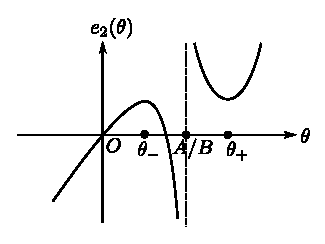
\includegraphics{vol79-fig/fig79-14.eps}
\smallskip
\caption{}
\label{chap2-fig2.1}        
\end{figure}\pageoriginale

Thus $\rho_2 (\theta)$ has a maximum at $\theta = \theta_- \varepsilon
(0.1)$ and a minimum at $\theta_+ > A/B$ which are easily determined to
be : 
$$
\theta_\pm = \frac{A}{B}\{ 1 \pm(1- B/A)^{1/2}\} 
$$

The maximum is thus: 
$$
\rho_{2_{\max}} = \rho_2(\theta_-) = \frac{[1-
    \frac{A}{B}(1-(1-B/A)^{1/2})][1-(1-B/A)^{1/2}]}{B(1-B/A)^{1/2}} 
$$

We write:
$$
\frac{A}{B}= 1 + \frac{1}{\varepsilon},\quad\text{where}\quad
\frac{1}{\epsilon}= \frac{M_0 K_0 K_1}{K_2}  
$$

Then if $\in$ is small, say $0 < \in << 1$, we have the expansion:
\begin{gather*}
\theta_- = \frac{1}{2}+ \frac{\varepsilon}{8}+\cdots\cdots,
\tag{2.17a}\label{chap2-sec2.14-eq2.17a}\\
 \rho_{2_{\max}} = \frac{1-(\varepsilon^2 /16)+\cdots\cdots}{(4M^2_0
   K_0 K_1 + 2M_0 K_2) - (M_0 K_2/2)\varepsilon + \cdots\cdots} \tag{2.17b} 
\label{chap2-sec2.14-eq2.17b}        
\end{gather*}

We\pageoriginale recall that $M_0 = \| (G_u^0)^{-1}\|$. Then if
$G_u^0$ becomes singular during continuation, $M_0$ becomes infinite
and the  continuation procedure explained here must fail. We notice this
phenomenon first by the required step sizes getting smaller. Also note
that small steps result from larger $K_0$, $K_1$ and $ K_2$ as well.  

In the implicit function theorem, we assumed that there is a solution
$(u^0 , \lambda^0)$. Next we prove a similar theorem in which we
assume only that $\| G(u^0, \lambda^0)\|$ is small.  

\setcounter{section}{17}
\section{Approximate Implicit Function Theorem}\label{chap2-sec2.18}

\textit{Let $G : B_1 \times B_2 \to B_1$ satisfy for some $\delta > 0$,
  $\rho_1 > 0$, $\rho_2 > 0$ sufficiently small}: 
\begin{equation*}
\begin{array}{r@{\;\;}>{$}p{7.5cm}<{$}}
\text{(a)} & \| G(u^0, \lambda^0) \| \leq \delta
\text{ \ for some \ } u^0 \in B_1, \lambda^0 \in B_2.\\
\text{(b)} & G^0_u \text{ \ is invertible and \ } \| (G^0_u) \|~\leq~M_0\newline \text{ \ for some constant \ } M_0.\\ 
\text{(c)} & G \text{ \ and \ } G_u \text{ \  are continuous on \ }
B_{\rho_1}(u^0) \times B_{\rho_2}(\lambda^0).
\end{array}\tag{2.18}\label{chap2-sec2.18-eq2.18}
\end{equation*}

\textit{Then there exist $u(\lambda)$,  for all $\lambda
  \in B_{\rho_1}(u^0)$, such that}:

\begin{center}
\begin{tabular}{r@{\;\;}>{$}p{9cm}<{$}}
(d) & G(u(\lambda ), \lambda ) =0 \textit{ \ and \ }
  u(\lambda)\in(U^0) 
  B_{\rho_1} (u^0) \text{ \ [Existence]}.\\ 
(e) & \text{For a given \ } \lambda \in
  B_{\rho_2}(\lambda^0) \text{  \ there is no solution of \ }\newline G(u,
  \lambda) = 0 \text{ \ in \ } B_{\rho_1} (u^0) \text{ \ other than
    \ } u(\lambda) \text{ \  [uniqueness]}.\\
(f) & u(\lambda) \text{ \ is continuous on \ } B_{\rho_2}(
  \lambda^0) \text{ \ and has the same modulus}\newline \text{of continuity as \ } G_u(u,
  \lambda)  \text{ \ [continuity]}.
\end{tabular}
\end{center}

\begin{proof}
We can prove the result in the same way as we have proved the implicit
function theorem. Since $G^0_u$ is nonsingular, the problem $G(u,
\lambda)= 0$ reduces to the fixed point problem  
$$
u= F(u, \lambda). 
$$\pageoriginale
where 
$$
F(u,\lambda)= (G^0_u)^{-1} [G^0_u u - G(u, \lambda)].  
$$

New for $\lambda \in B_{\rho_2}(\lambda^{0})$, we have: 
$$
\|u^0 - F (u^0 , \lambda)\| \leq \| u^0 - F (u^0, \lambda^0)\| + \| F
(u^0, \lambda^0) - F (u^0, \lambda)  \|,  
$$
and so: 
\begin{equation*}
\| u^0 - F(u^0, \lambda) \| \le M_0 (\delta +
\omega_0(\rho_2)). \tag{2.19a}\label{chap2-sec2.18-eq2.19a} 
\end{equation*}

Here $\omega_0$ is given by \eqref{chap2-sec2.7-eq2.10}(2.10). Next,
for $u$, $v \in B_{\rho_1}(u^0)$:  
$$
F(u,\lambda)- F(v, \lambda)= (G^0_u)^{-1} [G^0_u-\widetilde{G}_u (u, 
  v,\lambda)] (u-v),  
$$
where $\widetilde{G}_u(u, v, \lambda)$ is defined as in
\eqref{chap2-sec2.7-eq2.11a}. Again using
(\ref{chap2-sec2.7-eq2.11b},c,d) we obtain:  
\begin{equation*}
\|F(u, \lambda)- F(v, \lambda)\| \leq M_0 (\omega_1 (\rho_1)+
\omega_2(\rho_2))\|u-v\|.\tag{2.19b} \label{chap2-sec2.18-eq2.19b}
\end{equation*}

Now for any $\theta \in (0, 1)$ , choose $\rho_1$ and
$\rho_2$, small enough, such that : 
\begin{equation*}
M_0(\omega_1 (\rho_1)+(\omega_2 (\rho_2)) \leq \theta < 1,
\tag{2.19c}\label{chap2-sec2.18-eq2.19c} 
\end{equation*}
and
\begin{equation*}
M_0 (\delta + \omega_0(\rho_2)) \leq (1-\theta)
\rho_1. \tag{2.19d}\label{chap2-sec2.18-eq2.19d} 
\end{equation*}

Now we can apply the contraction mapping theorem to obtain the results  
\end{proof} 

\setcounter{section}{19}
\section{Step Length Bound}\label{chap2-sec2.20}

We can also obtain step length bounds as before. Thus we assume
\eqref{chap2-sec2.14-eq2.15} to hold and use it
in \eqref{chap2-sec2.18-eq2.19d} to get   
$$
M_0(\delta + K_0 \rho_2) \leq (1 - \theta) \rho_1 
$$\pageoriginale

If we take :
\begin{equation*}
\rho_2=  \frac{(1-\theta)\rho_1 - M_0 \delta}{M_0 K_0}
\tag{2.21a}\label{chap2-sec2.20-eq2.21a}  
\end{equation*} 
then \eqref{chap2-sec2.18-eq2.19d} holds. Again from
\eqref{chap2-sec2.18-eq2.19c}, using \eqref{chap2-sec2.14-eq2.15} we
require: 		
\begin{equation*}
M_0 (K_1\rho_1+ K_2\rho_2)= \theta <
1. \tag{2.21b}\label{chap2-sec2.20-eq2.21b} 
\end{equation*}

Substituting the value of $\rho_1$ from
(\ref{chap2-sec2.20-eq2.21a},b) we get:  
$$
\widetilde{\rho}_2(\theta)= \frac{(1-\theta)\theta - C}{A-B \theta},  
$$
where,
$$
A=M^2_0 K_0 K_1+B = M_0 K_2, C=M_0^2 K_1\delta.  
$$
\noindent
$\widetilde{\rho}_2(\theta)$ is sketched in
fig.~\ref{chap2-fig2.2}. We see that
$\widetilde{\rho}_2(\theta)$ has a maximum at $\theta_-\in (0,1)$ and a
minimum at $\theta_+> A/B$ which are given by : 
$$
\theta_\pm = \frac{A}{B}\{1 \pm (1-B/A- (B^2/A^2)C)^{1/2}\}.
$$

The maximum is thus: 
$$
\widetilde{\rho}_{2 \max }= \widetilde{\rho}_2(\theta_{-}).
$$

We have $C > 0$ and $A-B \theta \geq 0$ if $\theta \leq A/B$. Hence
$\widetilde{\rho}_2 \max$ in this theorem is less than that in the
original implicit function theorem. We write: 
$$
\frac{A}{B}= 1+\frac{1}{\varepsilon},\quad \text{where}\quad
\varepsilon =  \frac{K_2}{M_0 K_0 K_1},  
$$
and  
$$
C= M^2_0 K_1 \delta = D\cdot \frac{1}{\varepsilon},
$$
where\pageoriginale $D= \dfrac{M_0 K_0 \delta}{K_0}$. If $\varepsilon$
is small say, $0< \varepsilon << 1$, then we have the expansions: 
$$
\theta_- = \frac{1}{2} (1+D) +  \frac{\varepsilon}{8} (1-D)^2 + \cdots\cdots,  
$$
and 
$$
\widetilde{\rho}_{2\max} = \frac{(1-D)^2 + \frac{D}{2}(1-D)^2
  \varepsilon 
-   \frac{1}{8}(1-D)^4 \varepsilon^2 + \cdots\cdots}{(4M^2_0 K_0 K_1 +
  2M_0 K_2 - 2M_0 K_2 D ) - \frac{M_0 K_2}{2}(1-D)^2 \varepsilon + \cdots\cdots}  
 $$

Again as before, we can see that $\widetilde{\rho}_{2 \max}$ is small if
$M_0$ is large. Note that $\widetilde{\rho}_{2 \max}$ is always less than
$\rho_{2\max}$ in the implicit function theorem.  

\begin{figure}[H]
\centering
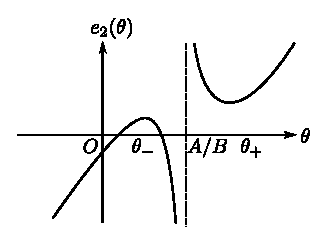
\includegraphics{vol79-fig/fig79-15.eps}
\smallskip
\caption{}
\label{chap2-fig2.2}
\end{figure}

\setcounter{section}{21}
\section{Other Local Rootfinders}\label{chap2-sec2.22}%%% 2.22 

Let  $g : \mathbb{R}\to \mathbb{R} $ be a smooth function. We will
examine various methods for finding the roots of $g(x) = 0$. In
particular, we consider the  chord method, Newton's method etc. In the
chord method, we choose an initial estimate $x_0$ of the solution and
a slope a. Then the line with slope `$a$' through $(x_0, g(x_0))$ will
intersect the $x$-axis at $x_1$. This is the next approximation to
the solution. We continue the process with $x_1$ replacing\pageoriginale $x_0$,
using the same slope `$a$' (See Fig.~\ref{chap2-fig2.3}). More precisely,  
$$
a(x_1 - x_0) = -g(x_0)
$$
and in general  
$$
a(x_{k+1} - x_k)= - g (x_k) 
$$

The sequences $\{ x_k \}$ thus generated, converges to a zero $g(x)$ if,  
$$
\max_{x \in H} \left| 1- \frac{g'(x)}{a} \right| <1,
$$
where $H$ is an interval containing both the initial value and a root
of the equation.  
\begin{figure}[H]
\centering
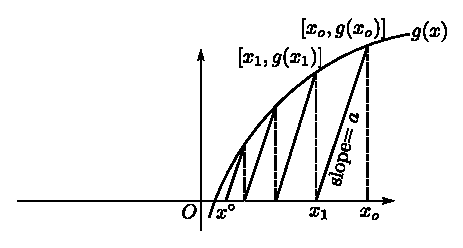
\includegraphics{vol79-fig/fig79-16.eps}
\smallskip
\caption{}
\label{chap2-fig2.3}
\end{figure}

In the higher dimensional case, we generalize the above to get the
sequence $\{ u_U \}$, form:  
$$
A[u_{U+1} - u_{U}]= -G(u_U),   
$$
where $G : \mathbb{R}^n \to \mathbb{R}^n$ and $A$ is an $n\times n$ 
matrix. In particular if we use:  
$$
a= g'(x_0) \text{ and } A= G_u(u_0),   
$$\pageoriginale
we get the special Newton method.  

In Newton's method we vary the slope at each iterate and take : 
\begin{align*}
a_U &= g'(x_U) \\
A_U &= G_U(u_U). 
\end{align*}

The Newton-Kantorovich theorem gives conditions under which the Newton
iterate converge.  


\section{Newton-Kantorovich Theorem}\label{chap2-sec2.23}%%% 2.23

\textit{Let} $G : B \to B$ ($B$ is a Banach space) \textit{satisfy for some
$u^0 \in B$ and $\rho^-_0 > 0$:} 
\begin{equation*}
\begin{array}{r@{\;\;}l}
\text{(a)} & G_u (u^0) \text{ \ is nonsingular with \ } \|
  (G^0_u)^{-1}\| \leq \beta;\\  
\text{(b)} & \| G_u^-1(u^0) G (u^0) \| \leq \alpha;\\  
\text{(c)} & \| G_u(u) - G_u(v) \|\leq \gamma \| u-v \|, \text{ \ in
  for all \ } u, v \in B_{\rho^-_0} (u^0) \, \backslash \, \{ (u^0) \}\\  
\text{(d)} &  \alpha \beta \gamma \leq \dfrac{1}{2} \text{ \ and \ }
\rho^-_{0} \leq \dfrac{1 - \sqrt{1 - 2 \alpha \beta
    \gamma}}{\beta\gamma}.
\end{array}\tag{2.23}\label{chap2-sec2.23-eq2.23}
\end{equation*}

\textit{Then the Newton iterates $\{u_U\}$ defined by Newton's
  method}:
$$
G_u(u_U) [u_{U+1} - u_U] = - G(u_U), U = 0,1,2, \ldots\ldots
$$ 
\textit{with \ $u_0 = u^0$ \ satisfy}:
\begin{equation*}
\begin{array}{r@{\;\;}>{$}p{8cm}<{$}}   
\text{(e)} & u_U \in B_{\rho^-_0} (u^0).\\   
\text{(f)} & \{ u_U\} \text{ \ converges to $u^*$, a root of \ }
  G(u)= 0 \text{ \ in \ } B_{\rho^+_0} (u^0).
\end{array}\tag{2.23}\label{chap2-sec2.23-addeq2.23}
\end{equation*}

\textit{In addition\pageoriginale  $u^*$ is the is
  the unique root of $G$ in $B_{\rho^+_0} (u^0)$ where}
$$ 
\rho^+_0= (1+(1-2\alpha \beta \gamma )^{1/2})/\beta \gamma.
$$

\begin{proof}
See the reference \cite{key16}
\end{proof}

Now we prove a theorem, assuming the existence of a root, to show the
basic idea of how the above method works.  

\section{Newton Convergence Theorem}\label{chap2-sec2.24}%%% 2.24

\textit{Let $G: B \to B $ and $G(u)=0$ have a root
$u=u^{*}$.  For some $\rho_{*} > 0$ let $G$ satisfy}: 
\begin{equation*}
\begin{array}{r@{\;\;}l}
\text{(a)} & \| G^{-1}_{u} (u^{*}) \| \leq \beta.\\ 
\text{(b)} & \| G_u(u)-  G_u(v) \| \leq \gamma \| u-v \|,
\textit{ \ for all \ } u, v \in B_{\rho_{*}} (u^{*}).\\ 
\text{(c)} & \rho_{*} \beta \gamma < \dfrac{2}{3}.
\end{array}\tag{2.24}\label{chap2-sec2.24-eq2.24}
\end{equation*}
 
\textit{Then for every $u_0 \in B_{\rho_{*}} (u^{*})$ the
  Newton iterates satisfy}:
\begin{equation*}
\begin{array}{r@{\;\;}l}  
\text{(d)} & u_U \in B_{\rho_{*}}( u^{*});\\
\text{(e)} & \| u_{U+1} - u^{*}\| \leq a \| u_U - u^{*}\|^2;  
\end{array}\tag{2.24}\label{chap2-sec2.24-addeq2.24}
\end{equation*}
\textit{where}, 
$$
a \equiv \frac{B\gamma}{2(1-\rho_* \beta \gamma)}< \frac{1}{\rho _*}. 
$$

\begin{proof}
For any $u \in B_{\rho_*} (u^{*})$ we have the identity :  
$$
G_u(u ) = G_u(u^* )\{ I+G_u^{-1} (u^* ) [G_u(u )-G_u(u^* )]\}.  
$$

Then (\ref{chap2-sec2.24-eq2.24}a,b,c) imply that:  
$$
\| G_u^{-1}(u^*)[G_u(u )-G_u(u^* )]\| \leq \rho_* \beta \gamma <
\frac{2}{3}.  
$$

Hence,\pageoriginale by the Banach lemma, $\{ I+G_u^{-1} (u^* )
[G_u(u)-G_u(u^*)]\} $ is invertible and so is $G_u(u)$. From the same 
lemma we get the estimate : 
  \begin{equation*}
\| G^{-1}_u (u) \| \leq \frac {\beta}{1-\rho_* \beta
  \gamma}. \tag{2.25}\label{chap2-sec2.24-eq2.25} 
  \end{equation*}  
 
Now we will prove by induction that $u_U \in B_{\rho_*}(u^*)$,
 $u= 0, 1, 2, \ldots $. Suppose $u_U \in B_{\rho_*}(u^*)$. Then  
 $$
 u_{U+1} - u^* = (u_U- u^*)-  G_u^{-1} (u_U)[G(u_U)- G(u^*)]. 
 $$
 
 By the mean value result \eqref{chap2-sec2.5-eq2.6}, we have : 
 $$
 G(u_U)- G(u^*) = \widetilde{G}_u(u_U, u^*)(u_U - u^*),  
$$
and so: 
$$
u_{U+1} - u^* = G^{-1}_{u} (u_U) [G_u (u_U) - \widetilde{G}_u (u_U,
u^*)] (u_U - u^*).  
$$

But 
\begin{align*}
\| G_u (u_U) - \widetilde{G}_u (u_U, u^*)\|
  & \leq \int\limits^1_0 \| G_u
  (u_U)- G_u (tu_U+(1-t)u^*)\| \, dt\\  
  & \leq \gamma \int\limits^1_0 \| ( 1-t)(u_U - u^*)\| \, dt\\ 
  &\qquad = \frac{\gamma}{2} \| u_U - u^* \|.
\end{align*}
  
  Hence 
\begin{equation*}
  \begin{split} 
  \| u_{U+1} - u^*\|  & \leq \| G_u^{-1}(u_U)\|. \frac{\gamma}{2}\| u_U
  - u^*\|^2, \\ 
    & \leq \frac{\beta}{1-\rho_*\beta \gamma} \frac{\gamma}{2} \| u_U -
  u^* \|^2, 
  \end{split}\tag{2.26}\label{chap2-sec2.24-eq2.26}
\end{equation*}
  by \eqref{chap2-sec2.24-eq2.25}. Note that   
  $$
  \frac{\beta \gamma}{2(1-\rho_* \beta \gamma)} \leq \frac{1}{\rho_*} 
  \text {and } \| u_U-u^* \| \le \rho_*.   
   $$

  Hence\pageoriginale $u_{U+1} \in B_{\rho_*}(u^*)$ and by induction (d)
  follows. Then (e) follows from \eqref{chap2-sec2.24-eq2.26}. 
\end{proof}

\begin{note*}
The convergence here, is quadratic. Thus if 
$$
a\| u_U - u^* \| \leq 10^{-p_U}
$$
for some positive $p_U$, then 
$$
a\| u_{U+r}-u^*\| \leq 10^{-2^u \rho_U } \| u_U - u^* \| \text { for 
  any } r = 0, 1,2, \ldots\ldots.  
$$
\end{note*}

The choice of  the initial iterate, $u_0$, is important in using
Newton's method. It is not uncommon to spend 90\% or more of the
effort in finding a food approximate value of the root. Our study will
show many ways in which such difficulties can be overcome. Another
problem with Newton's method can be the time it takes to solve
the linear system for the new iterate. This occurs, for example, if
$B = \mathbb{R}^N$ for very large $N$, say $N \approx 10^3$ or larger (when
approximating nonlinear P.D.E. problems). The so called
\textbf{quasi-Newton methods} are designed to avoid the linear system
problem by some device (for example updating secant method, which we
are going to describe in the next section). 


\setcounter{section}{26}
\section{Predictor-Solver Methods}\label{chap2-sec2.27}%%% 2.27

Let $G: \mathbb{R}^N \times \mathbb{R} \to \mathbb{R}^N$. At the root $(u^0,
\lambda^0)$ of $G(u, \lambda) = 0 $, let $G^0_{u}$ be
nonsingular. Then the implicit function theorem shows the existence of
the unique branch of solutions $u = u(\lambda)$ in a neighbourhood of
$\lambda^0$. We will briefly describe various \textbf{predictor-sovler
  methods} for determining $u (\lambda)$. These proceed by using the
solution $(u^0, \lambda)$. to construct a better approximation
$u_0(\lambda)$ to the actual solution $u(\lambda)$. This is the
predictor.  
After\pageoriginale obtaining the initial approximation, we apply an iteration
scheme for which the sequence of iterates converges to the solution
$u(\lambda)$. This is the solver. 

\subsubsection*{Various Predictors}

\begin{enumerate}[(i)]
\item {\bf Trivial Predictor} : Here we take the initial approximation
  as (see (Fig.~\ref{chap2-fig2.4}a)): 
$$
u_0 (\lambda) = u^0 = u (\lambda^0) 
$$   
i.e. the initial guess at $\lambda$ is equal to the solution at
$\lambda^0$. The error estimate is given by : 
\begin{align*}
|| u(\lambda ) - u_0 (\lambda ) || &= || u(\lambda ) - u(\lambda^0 )
||, \\ 
&\leq \frac{M_0}{1-\theta} \omega_0 (| \lambda - \lambda^0 |). 
\end{align*} 

Here $u(\lambda)$ is the actual solution and $\omega_0$ is given by
\eqref{chap2-sec2.7-eq2.10}. If $G(u, \lambda)$ is Lipshitz continuous
in $u$ then   
$$
|| u(\lambda ) - u_0 (\lambda) || \leq \frac{m_0}{1-\theta} K_0 |
\lambda - \lambda^0 |, 
$$ 
where $K_0$ is the corresponding Lipshitz constant. 

\item {\bf Secant-Predictor}: Here we assume that there are two known
  solutions $(u^0, \lambda^0)$ and $(u^1,\lambda^1)$. Then consider
  the line  segment joining $(u^0, \lambda^0)$ and $(u^1,\lambda^1)$
  in the $(u, \lambda)$ space. Take $u_0 (\lambda)$ as the point on
  this line with given $\lambda$-coordinate value $\lambda$. (See
  Fig.~\ref{chap2-fig2.4}b) i.e. 
$$
u_0 (\lambda ) = u^1 + (\lambda - \lambda^1) \frac{u^1 -
u^0}{\lambda^1 - \lambda^0}. 
$$

Then\pageoriginale 
\begin{align*}
u(\lambda ) - u_0(\lambda) & = [u(\lambda ) - u (\lambda^1 )] - \frac{\lambda -
  \lambda^1}{\lambda^1 - \lambda^0} [u(\lambda^1 ) - u (\lambda^0 )], 
\\ 
& = \tilde{u}_{\lambda}(\lambda ,\lambda^1 )  (\lambda - \lambda^1 ) -
(\lambda - \lambda^1 ) \tilde{u}_\lambda (\lambda^1 , \lambda^0 ). 
\end{align*}

By the mean value formula \eqref{chap2-sec2.5-eq2.6}: 
{\fontsize{10pt}{12pt}\selectfont
\begin{align*}
u(\lambda ) - u_0 (\lambda ) &= \int\limits_0^1  dt[u_\lambda
  + (1-t)\lambda^1 ) - u_\lambda (t \lambda^1 + (1-t)\lambda^0 )]
(\lambda - \lambda^1 ),\\ 
&= \int \limits_0^1  dt \int\limits_0^1 \{ u_{\lambda
  \lambda}  (s (t \lambda + (1-t)\lambda^1)  + (1-s)(t \lambda^1 + (1-t)
\lambda^0 ))\\
& \qquad (t(\lambda - \lambda^1 ) + (1-t)(\lambda^1 - \lambda^0 ))
(\lambda - \lambda^1 )\} ds. 
\end{align*}}\relax

Again we have use \eqref{chap2-sec2.5-eq2.6}. Thus we get:
\begin{align*}
|| u(\lambda ) -u_0 (\lambda ) || &\leq \frac{1}{2}K_2 [ (\lambda -
  \lambda^1 ) + (\lambda^1 - \lambda^0 )] (\lambda - \lambda^1 ),\\ 
&= \frac{1}{2}K_2 (\lambda - \lambda^0 ) (\lambda - \lambda^1 ),
\qquad \lambda^0 < \lambda^1 < \lambda , 
\end{align*}
where,
$$
K_2 = K_2 (\lambda) \equiv \max_{\tilde{\lambda} \in [\lambda^0,
    \lambda]} ||u_{\lambda \lambda }(\tilde{\lambda}) ||. 
$$

Since $\lambda^0 < \lambda^1 < \lambda$, this is an extrapolation.

In the interpolation case, that is , $\lambda^0 < \lambda <  \lambda^1$,
we have : 
$$
|| u(\lambda ) - u_0(\lambda) || \leq \frac{1}{2} K_2 (\lambda -
\lambda^0 )(\lambda^1 - \lambda ). 
$$

\begin{figure}[H]
\centering
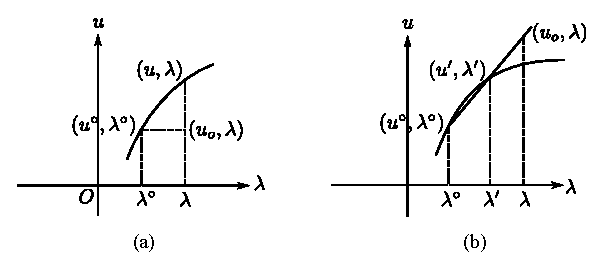
\includegraphics{vol79-fig/fig79-17.eps}
\smallskip
\caption{}
\label{chap2-fig2.4}
\end{figure}

\item {\bf Higher-order Predictor (Lagrange)}:\pageoriginale If we
  know more than 
  two solutions, then we can take higher order approximations to the
  next solution by using order interpolation formulae. 

\item {\bf Tangent Predictor (Euler method)}: In the secant predictor
  meth\-od we assumed the existence of two solutions and then used the
  line segment joining these two solutions. Now we will consider only
  the solution at a single point and use the tangent to the solution
  curve at that point. (see Fig.~\ref{chap2-fig2.4c}). From the
  implicit function theorem we have: 
$$ 
G(u (\lambda),\lambda) = 0 \text{ for all } \lambda \in
B_{\rho_2} (\lambda^0). 
$$ 

Differentiating with respect to $\lambda$, we get: 
$$
G_u(u(\lambda ),\lambda ) \dot{u} (\lambda) = - G_\lambda (u(\lambda
),(\lambda ), 
$$
and thus
$$
\dot{u}^0 =  \dot{u}(\lambda^0 ) = - (G^0_u )^{-1}G^0_\lambda. 
$$

Then we take the approximation as :
$$
u_0(\lambda ) = u^0 + (\lambda - \lambda^0) \dot{u}^0. 
$$

The error is given by:
$$
u(\lambda ) - u_0(\lambda ) = \frac{1}{2} \ddot{u}^0(\lambda -
\lambda^0 )^2 + 0 ((\lambda - \lambda_0)^3 ). 
$$
\end{enumerate}


\setcounter{figure}{3}
\begin{figure}[H]
\centering
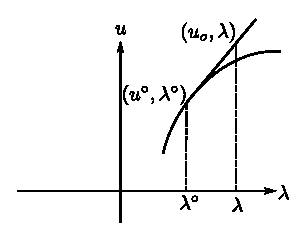
\includegraphics{vol79-fig/fig79-18.eps}
\smallskip
\caption{(c)}
\label{chap2-fig2.4c}
\end{figure}

\noindent
\textbf{Solvers}: Now\pageoriginale using predictor $u_0(\lambda )$,
our aim is to 
construct an iteration scheme of the form  
$$
A_U (u_{U+1} - u_U) = - G(u_U, \lambda ), U = 0,1,2, \cdots \cdots ,  
$$
where $\{A_U\}$ are suitable matrices which assure the convergence of
$\{u_U\}$ to a root 
\begin{enumerate}[(i)]
\item {\bf Special Newton Method}  

In the special special Newton method, $A_U$ is given by the constant
operator $G^0_u$. 
 
 \item {\bf Newton's Method}
 
 In Newton's method, $A_U \equiv G^U_u = G_u(u_U, \lambda )$. One of
 the important advantages of Newton's method is that it can have
 quadratic convergence i.e. the sequence $(u_U)$ satisfies : 
 $$
 || u_{U+1} -u^*  || \leq \beta || u_U - u^*  ||^2, 
 $$ 
 for some constant $\beta$, where $u^*$ is the actual solution.
 

 \item {\bf Updating-Secant Method}

 As mentioned above a major disadvantage of Newton's method is that
 we need to solve a linear system with the coefficient matrix $G^U_u$
 step $U = 0,1,2, \ldots \ldots$. This costs $0(N^3)$ operations at
 each step, where $N$ is the dimension of the space. 
 \end{enumerate}
 
 Now we will introduce \textbf{Updating-Secant Method.} The idea of this
 iteration scheme is to obtain a suitable approximation $A_U$ to
 $G^U_u$ so that\pageoriginale the system at $(U+1)^{st}$ stage can easily be
 solved if we can solve the system at $U^{th}$ stage. Further
 $A_{U+1}$ is to satisfy a relation also satisfied by $G^{U+1}_u$. We
 will take $A_{U+1}$ in the form: 
 \begin{equation*}
A_{U+1} = A_{U}+ C_UR_U^T, \tag{2.28}\label{chap2-sec2.27-eq2.28}
  \end{equation*}  
  where $C_U$ and $R_U$ are column vectors of dimension $N$ and $A_U$
  is an $N \times N$ matrix. In particular we choose: 
  $$
  C_U \equiv \frac{(y_U - A_U S_U)}{< S_U, S_U>}, 
  $$
  and  
  $$
  R^T_U \equiv S^T_U,
  $$
  where 
  $$
  y_U = G(x_{U+1}) - G(x_U) \text{ and } S_U = x_{U+1} - x_U.  
  $$

  Now we have to solve the linear system $A_US_U = - G(x_U)$ at each
  step. But this can be easily achieved using the Shermann-Morrison
  formula [for more details see \cite{key12}). 

\setcounter{section}{28}
\section{Lemma}\label{chap2-sec2.29}%%% 2.29

Let A be an  $N \times N$ invertible matrix and  $u$, $v \in
    \mathbb{R}^N$. Then $A+uv^T$ is nonsingular if and only if
    $\sigma = 1+(v, A^{-1} u)\neq 0$, and then the inverse of
    $(A+uv^T)$ is given by 
  \begin{equation*}
(A+uv^T)^{-1} = A^{-1} - \frac{1}{\sigma} A^{-1}uv^TA^{-1} \tag{2.29a} 
\label{chap2-sec2.29-eq2.29a}
\end{equation*}  

Using this result and \eqref{chap2-sec2.27}, the inverse of $A_{U+1}$
is given by   
  \begin{equation*}
A^{-1}_{U + 1} = A^{-1}_U + \frac{(s_U - A_U^{-1} y_U) s^T_U
  A^{-1}_U}{(s_U, A_U^{-1}y_u)} \tag{2.29b} \label{chap2-sec2.29-eq2.29b}
\end{equation*}\pageoriginale  

This method uses only $0(N^2)$ arithmetic operations. Naturally, we
can expect a loss in the rate of convergence compared to Newton's
method here we get only \textit{superlinear convergence} instead of
quadratic convergence. i.e.  
$$
|| u_{U+1} - u^* || \leq \alpha_U || u_U - u^* ||  
$$
where 
$$
\alpha_U \to 0 \text{ as } U \to \infty 
$$

This is generally  known as a Quasi-Newton method (see ref: \cite{key9}).  

